\documentclass[11pt,a4paper]{article}
%\usepackage{beamerarticle}

%\usefonttheme[onlymath]{serif}
\usepackage[ngerman]{babel}
\usepackage[utf8]{inputenc}
\usepackage[T1]{fontenc}
\usepackage{tikz}
\usetikzlibrary{positioning, arrows}
\usepackage{listings}
\usepackage{fancybox}
\usepackage{color}
\usepackage{hyperref}
\usepackage{fancyhdr}

\pagestyle{fancy}
\lhead{\today}
\author{Gruppe: SWT15-GKP}
\rhead{Author: PP,FB}
\chead{Gruppe: SWT15-GKP}
%\cfoot{center of the footer!}
\renewcommand{\headrulewidth}{0.8pt}
%\renewcommand{\footrulewidth}{0.4pt}
\title{Universität Leipzig - Softwaretechnik Praktikum 2014/2015 \\  Entwurfsbeschreibung zum Vorprojekt \\ zum Projekt: Ein kartenbasiertes “Multiplayer”-Spiel}

\begin{document}
\maketitle

\clearpage

\tableofcontents

\clearpage

\flushleft
\section{Allgemeines}
Im Rahmen des SWT-Praktikums wird ein kartenbasiertes Multiplayerspiel entwickelt, das es ermöglicht, ein an das alte Pacman angelehnte Computerspiel auf einem realen Kartenausschnitt zu spielen. \\
Im Vorprojekt wird eine kleine Web Applikation erstellt, welche die Architektur minimal implementiert und eine einfache Interaktion mit der Karte ermöglicht.
Genauer gesagt ist es möglich einen Spielort auszuwählen und dort mit einer Spielfigur über den Kartenausschnitt zu laufen, sowie mit einer weiteren Spielfigur zu interagieren.


\section{Produktübersicht}
Der Nutzer kann online über die Spiele-Website auf das Programm zugreifen.
Dabei stehen dem Nutzer ein Suchfeld zum finden der gewünschten Spielumgebung zur Verfügung, die Möglichkeit die Spielfigur zurück zusetzen und die Lautstärke über einen Regler anzupassen. \\
Hat man den Ort ausgewählt, kommt eine weitere Spielfigur (der Geist) ins Spiel, die sich zufallsgeneriert über die Karte bewegt. \\
Man kann die Spielfigur, den Pucman, nun steuern und wenn man es schafft mit Pucman den Geist einzufangen, wird ein Geräusch ausgelöst. \\
Während des Spielens werden die Möglichkeiten zur Veränderung der Kartenansicht deaktiviert um sicherzustellen, dass der Spieler sich nicht unabsichtlich vom Spielgeschehen entfernen kann. \\
Das ganze Spielgeschehen ist durch einen Soundtrack unterlegt, der eine  funktionale und inhaltliche Verbindung zwischen Bild und Musik  generiert. \\
Desweiteren befinden sich bereits Platzhalter für den späteren Highscore, die verbleibende Anzahl an Leben und die Möglichkeit direkt auf die Website des Spiels zugreifen zu können.
\clearpage
\section{Grundsätzliche Struktur- und Entwurfsprinzipien}
Als grundsätzliche Programmiersprache haben wir uns für Java-Script entschieden. Wobei der Java-Scriptcode von einer html-Seite aufgerufen wird. Vielleicht nehmen  wir auch Phaser. \\
Die von uns umgesetzte Web-Anwendung basiert auf einer Client-Server Architektur. Wir arbeiten also mit einem Html-Server auf dem die Daten liegen, die vom Client abgefragt und an diesen übertragen werden. Diese Daten beinhalten auch den Gameblock, der dann vom Client ausgeführt wird. Darüber hinaus arbeiten wir mit der Googlemaps API, die alle wichtigen Funktionen zur Manipulation der Karte zur Verfügung stellt.\\
\begin{figure}[htb]
  \centering
  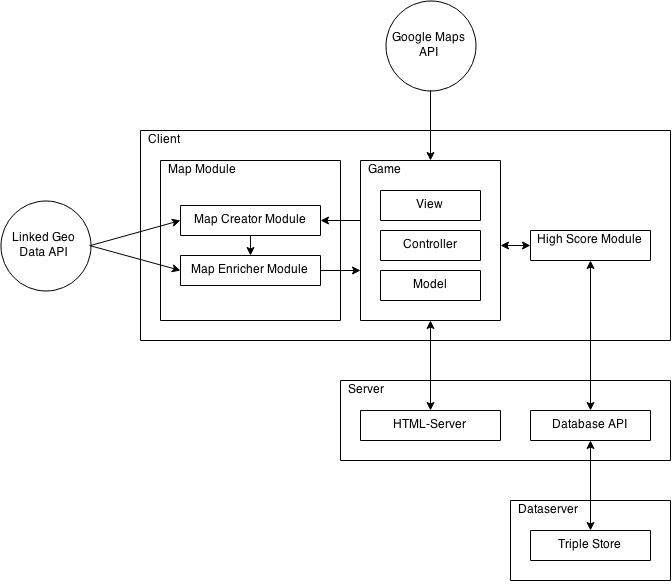
\includegraphics[scale=0.4]{arch.png}
%\caption{der rote Punkt bezeichnet unser gesuchtes Teilwort}
  \label{PNFs}
\end{figure} 



\section{Struktur- und Entwurfsprinzipien der einzelnen Pakete}
\subsection{Server} Vom Server werden die benötigten Spieldatein zur Verfügung gestellt und automatisch geladen.

\subsection{Client - Gameblock}
Der Gameblock wird an das Model-View-Controller Prinzip angelehnt, welches durch die Nutzung von Phaser umgesetzt wird. \par\bigskip
\begin{figure}[htb]
  \centering
  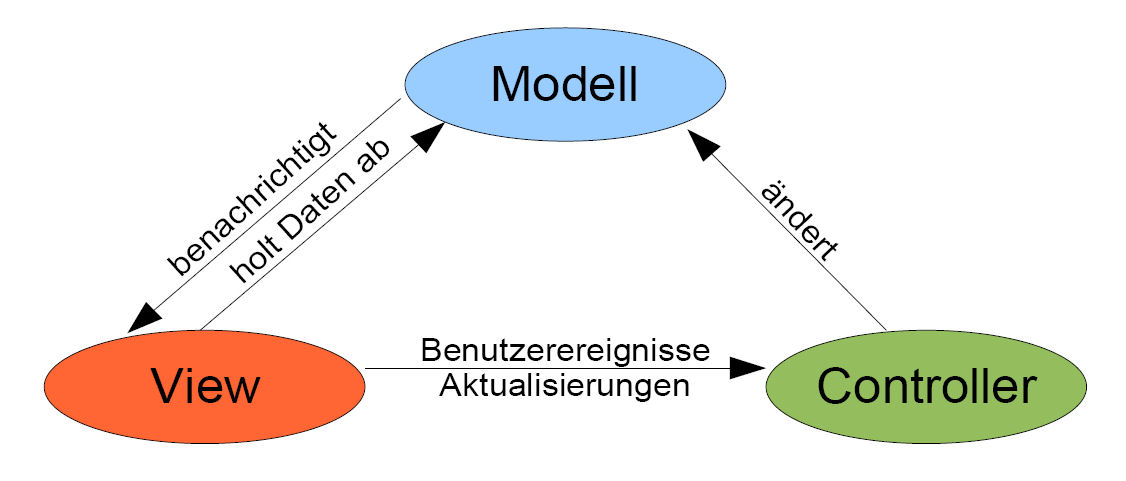
\includegraphics[scale=0.2]{mvc.jpg}
%\caption{der rote Punkt bezeichnet unser gesuchtes Teilwort}
  \label{PNFs}
\end{figure} 

%\clearpage 



\textbf{Modell (model)} \\
Das Modell enthält die darzustellenden Daten und ist von Präsentation und Steuerung unabhängig. Das Modell ist das zu beobachtende Subjekt.\\

\par\bigskip \par\bigskip
\textbf{Präsentation (view)} \\
Die Präsentationsschicht ist für die Darstellung der benötigten Daten aus dem Modell und die Entgegennahme von Benutzerinteraktionen zuständig. Sie kennt sowohl ihre Steuerung als auch das Modell, dessen Daten sie präsentiert, ist aber nicht für die Weiterverarbeitung der vom Benutzer übergebenen Daten zuständig. \\

\par\bigskip \par\bigskip
\textbf{Steuerung (controller)} \\
Die Steuerung verwaltet die Präsentation, nimmt von ihr Benutzeraktionen entgegen, wertet diese aus und agiert entsprechend. Die Steuerung sorgt dafür, dass Benutzeraktionen wirksam werden, z. B. durch Änderung der Präsentation (z. B. Richtungsänderung von Pucman) oder  durch Weiterleiten an das Modell (z. B. Übernahme von Eingabedaten oder  Auslösen von Verarbeitungen). Die Steuerung beschränkt sich darauf Benutzereingaben (Daten und Methodenaufrufe) von der Präsentation an das Modell weiterzuleiten und enthält weiterhin Mechanismen, um die Benutzerinteraktionen der Präsentation einzuschränken.

\subsection{Google Maps API}

Das Herzstück der Anwendung ist die Googlemaps Api, die das Anzeigen der Karte  übernimmt.\\
Die folgenden integrierten Steuerelemente sind bei der Suche nach einem geeigneten Spielort verfügbar, danach werden die Elemente deaktiviert um einen flüssigen Spielbetrieb zu gewährleisten. \par\bigskip
Das \textbf{Zoomsteuerelement} zeigt für große Karten einen Schieberegler und für kleine Karten kleine Schaltflächen "+" und "-" an, damit die Zoomstufe der Karte gesteuert werden kann. Dieses Steuerelement wird auf berührungslosen Geräten standardmäßig links oben auf der Karte angezeigt bzw. unten links auf Geräten mit Berührungssteuerung.\par\bigskip
Das \textbf{Kartentyp-Steuerelement} ermöglicht das Umschalten zwischen Kartentypen, wie z. B. ROADMAP und SATELLITE. Dieses Steuerelement wird standardmäßig rechts oben auf der Karte angezeigt.\par\bigskip
Das \textbf{Schwenksteuerelement} zeigt Schaltflächen zum Schwenken der Karte an. Dieses Steuerelement wird auf berührungslosen Geräten standardmäßig links oben auf der Karte  angezeigt. Mit dem Schwenksteuerelement können Sie 45$^\circ$ -Bildmaterial drehen, sofern verfügbar.


\section{Datenmodell}
Für das Vorprojekt benutzen wir keine Daten, mit außnahme der Sound- und Bild-Dateien, welche sich auf dem Server befinden, und der Karte, die uns die Google Maps API liefert.

\section{Testkonzept}
Alle nötigen Funktionen werden von der Google Maps Api bereitgestellt.
Aufgrund des einfachen Programmaufbaus verzichten wir daher für das Vorprojekt auf ein besonderes Testkonzept und führen stattdessen manuelle Tests in Hinsicht auf die Funktionalität durch.
\section{Glossar}
Das Glossar wurde überarbeitet und als externes Dokument angefügt.
Die folgenden Begriffe und Konzepte wurden aufgenommen: \\
Jasmine, JamJS, Bower, HTML, CSS, Google Maps API, MVC, Versionskontrollsystem, KML Layer, Client, Server, Phaser, Open-Source.
\end{document}